Mixture models are one of the very first ideas applied in semi-supervised learning.  In this chapter, we directly derive the mixture model to the text data with the assumption of many components in the label conditional distribution and consider how we initialize these components.

\section{Problem Statement}
We are given a set of independently and identically distributed data $\mathcal{D} = \{\mathcal{D}_L, \mathcal{D}_U\}$ which consists of two subsets of labeled data $\mathcal{D}_L$ and unlabeled data $\mathcal{D}_U$. Denote that the number of labeled data $|\mathcal{D}_L| = l$ and unlabeled data $|\mathcal{D}_U| = u$. We always have the condition $u \gg l$. 

The labeled set has the form of pairs of data instances and its corresponding label, $\mathcal{D}_L = \{ (x^{(1)}, y^{(1)}), ..., (x^{(l)}, y^{(l)}) \}$, and the unlabeled set only contains the instances, $\mathcal{D}_U = \{ x^{(l+1)}, ..., x^{(l+u)} \}$. In addition, we denote the set of labeled instances $\mathcal{X}_L = \{ x^{(1)}, ..., x^{(l)} \}$ and the set of unlabeled instances $\mathcal{X}_U = \{ x^{(l+1)}, ..., x^{(l+u)} \}$, then the set of data instances $\mathcal{X} = \mathcal{X}_L \cup \mathcal{X}_U $. Correspondingly we have the set of labels $\mathcal{Y}_L = \{ y_1, ..., y_l \}$ for $\mathcal{X}_L$, the set of true label $\mathcal{Y}_U = \{ y_{l+1}, ..., y_{l+u} \}$ for $\mathcal{X}_U$ and the set of data label $\mathcal{Y} = \mathcal{Y}_L \cup \mathcal{Y}_U$.

This thesis only focuses on binary classification problem where the labels in $\mathcal{Y}$ only receive positive or negative value. Precisely, we have the condition $\mathcal{Y} \in \{-1,+1\}^{l+u}$. Hence the task is looking for an inference $\mathcal{X} \rightarrow \mathcal{Y}$ with inductive learning and estimating $\{ \mathcal{X}, \mathcal{Y}_L \} \rightarrow \mathcal{Y}_U$ with transductive learning.

\section{Mixture of Components for Text Data}
Suppose we are given the joint density distribution $P(\mathcal{X})$ with the unknown parameter set $\theta$ that we want to estimate through the observed data set $\mathcal{D}$. The distribution $P(\mathcal{X})$ has the form of a mixture of different independent components. Denote that the set of these components is $M$, then we have
\begin{align}
	\label{equal2: general many-to-one assumption}
	P(\mathcal{X}) = \sum_{M_j \in M}{P(\mathcal{X} | \theta_j) P(M_j)}
\end{align}
where $\theta_j \in \theta$ is the parameters of component $M_j$.

Now we want to look for the correspondent between $M$ and the label values $\{-1, +1\}$. The first idea here is that each component is equivalent with a label value \parencite{10.2307/2984875}, thus we have two components and directly express the distribution through the label value set as in (\ref{equal1: mixture of labels}). Then the extension to at least one component on a label value was generalized in \parencite{NIPS1996_1208}. So we have the predicted label of $y^{(i)}$ for the input data $x^{(i)}$ such that
\begin{align}
	\hat{y}^{(i)} = \argmax_{y \in \{-1, +1\}}{
		\sum_{M_j \in M}{P(y | M_j) P(x^{(i)} | \theta_j) P(M_j)}
	}
\end{align}

With the equivalent setting, \citeauthor{Nigam:2000:TCL:347709.347724} \parencite{Nigam:2000:TCL:347709.347724} was applying this model to the text data. We also adapted the term many-to-one assumption from there. The model is restricted that $P(y|M_j) \in \{0,1\}$ as the \textit{predefined components} on each label value, which means we have decided how many and which components are for each label value. Furthermore, the distribution of the components in the same label value $y$ is given and constrained of sum to equal to $1$, $\sum_{M_j : P(y | M_j)=1}{ P(M_j | y) } = 1$. Then we have the component mask
\begin{align}
	P(M_j|x) = P(M_j|y) P(y|x)
\end{align}

We are now reconstructing the model on text data and estimate the parameter for each component. Given a dictionary as list of ordered words $\textbf{w} = (w_1, ..., w_d)$ where $d$ is the number of different words in $\textbf{w}$. We represent the input as word count vector $x^{(i)} = \langle x_1^{(i)}, ...,x_d^{(i)} \rangle$ where each $x_k^{(i)}$ is the count of word $w_k$ in text $x^{(i)}$. Consider the joint density distribution of input data $x$ and component $M_j$, we have
\begin{align}
	P(x, M_j | \theta) = P(x | M_j, \theta) P(M_j|\theta)
\end{align}
with $x$ is assumed with the Naive Bayes assumption on the independence of word features. Hence what we have for component conditional is a multinomial distribution
\begin{align}
	P(x | M_j, \theta) = 
	(\sum_k{ x_k })! 
	\prod_{k=1}^{d}{ 
		\frac{
			P(w_k | M_j, \theta)^{x_k}
		}{
			x_k!
		}
	}
\end{align} 
On this step, with Naive Bayes assumption, there is one more different setup of Bernoulli distribution, where the word count feature be replaced by the word appearance---a word $w_k$ appears in $x$ or not. But it was empirically demonstrated that the Multinomial model has a better performance than the Bernoulli one \parencite{mccallum1998naive}.

We continue with the component prior distribution, which is frequently conjugated with a Dirichlet distribution. In this way, eventually, the estimate also assembles with the smoothing models \parencite{Chen1999}. So we set concentration parameters of the Dirichlet distribution with the same value and are equal to $2$ for a component prior distribution. This gives us an estimate with the uniform distribution and Laplace smoothing. So that
\begin{align}
	P(M_j|\theta) \propto \prod_{k=1}^{d} P(w_k | M_j, \theta)
\end{align}

So far we have specified the model for our components, we turn back to the estimator of $\theta$. Here we derive the maximum log-likelihood
\begin{align}
	\hat{\theta} = \argmax_{\theta}{\ln(P(\mathcal{D} | \theta))}
\end{align}
We first consider the basic case when there is only labeled data, the solution is straightforward with partial derivatives of Lagrangian with the constraint of $\sum_{k=1}^{d}{P(w_k | M_j)} = 1$. More details about the solution can be found in \parencite{Collins2013}. We have an estimate of the word conditional probability
\begin{align}
\label{equal2: all label conditional probabilities}
	P(w_k | M_j, \hat{\theta}) = \frac{
		\sum_{i=1}^{l}{x_k P(M_j|x)} + 1
	}{
		\sum_{k=1}^{d}\sum_{i=1}^{l}{x_k P(M_j|x)} + d
	}
\end{align}
and the prior probability
\begin{align}
\label{equal2: all label prior}
	P(M_j | \hat{\theta}) = \frac{
		\sum_{i=1}^{l} P(M_j | x) + 1
	}{
		l + 2
	}
\end{align}

Next we cooperate the data with the unlabeled set. In this case, we cannot directly solve the optimization of the log-likelihood and to only get to the local convergence using EM algorithm \parencite{10.2307/2984875}. Basically, the algorithm consists of two basic steps, the expectation (E-step) and the maximization (M-step). The process starts with an initial set of parameter, $\theta^{(0)}$. Then for each iteration, it repeatedly computes the E-step and M-step. At t-$th$ time, the E-step calculates the data conditional probability on the latent components for unlabeled data using the previously observed parameters $\theta^{(t-1)}$---the partial labels. After that at M-step, we would consider that our data have been temporally and partially labeled to components and estimate the parameter $\theta^{(t)}$ using (\ref{equal2: all label conditional probabilities}) and (\ref{equal2: all label prior}) correspondingly. The EM algorithm guarantees that the next parameter set $\theta^{(t)}$ is improved from $\theta^{(t-1)}$, which means we have the log-likelihoods $\ln(P(\mathcal{D}|\theta^{(t)})) \geq {\ln(P(\mathcal{D}|\theta^{(t-1)}))}$ \parencite{Borman2006}. Algorithm \ref{alg2: EM algorithm} presents the general framework of EM algorithm in our case. The convergence  condition could be the threshold of loop number or better is the different of log-likelihood between $\theta^{(t-1)}$ and $\theta^{(t)}$.

\begin{algorithm}[H]
	\caption{EM algorithm with labeled and unlabeled data}
	\begin{algorithmic}[1]
		\Function{EmAlgorithm}{$\mathcal{D}$}
		\State $t = 0$
		\State Initialize $\theta^{(0)}$
		\Repeat
		\State $t = t + 1$
		
		\State \texttt{\# E-step}
		\State $Q(x) \gets P(M | x, \theta^{(t-1)})$ 
						
		\State \texttt{\# M-step}
		\State $\theta^{(t)} \gets \argmax_{\theta} 
		{Q(x) \ln(P(x, M | \theta))}$ 
		
		\Until{$\theta^{(t)}$ is converged}
		
		\State \Return $\theta^{(t)}$
		\EndFunction
	\end{algorithmic}
	\label{alg2: EM algorithm}
\end{algorithm}

The initialization of $\theta^{(0)}$ setups the predefined component $P(y|M)$ for each label value and the label conditional on components $P(M_j|y)$. Basically, the predefined component is searched from an appropriate range of numbers and the problem left is the assignment of label conditional on components. We will discuss this in the next section.

\section{Component Initialization Problem}
Literally, the initialization step should be done by deciding the component number for each label value and assign labeled data for the components. The conventional method does it by randomly distributing the components probability throughout the label of the labeled instances. In this way, the only advantage of labeled data is restricted into the constraint on all components of its label and the same initialization is applied for all input components. Which means the inflexible with the change of data, in case of which we may upgrade the labeled set. The positive point of Naive Bayes is simple to implement and flexible with large amounts of data. Consequently, we should think about the methods that are not merely treating all the components in the same meaning, but elaborate the characteristics of input labeled set to enhance the learning model.

We may contemplate that the assignment of labeled data to components is an unsupervised task where we only know the component number. Here we derive two different unsupervised approaches to setup the assignment schemes. The first is constructing a hierarchical tree for each label value and the second is k-means clustering. These two are the basic clustering models of unsupervised learning, we can find a detailed description in \parencite{Manning:2008:IIR:1394399}. In this section, we only present their application with our model.

We begin with the hierarchical tree assignment. For each label value, we consider the similarity between components. A hierarchical clustering establishes and treats each cluster as a component using agglomerative structure. Figure \ref{fig2: tree assignment} gives the illustration of an agglomerative tree for a label value. The clustering processes through the iterated steps. From the beginning, each data instance is considered as a component. At each iteration, we merge the two most similar components until only one remains. We continuously index all components that are merged at each iteration as a layer. A component sampling will be done with the cutting process. A cut between two continuous layers $i$ and $j$ $(i < j)$ returns a set of assigned components. For example, the layer 3 and 4 are $\{\{1,2,3\},\{4\},\{5,6\}\}$ and $\{\{1,2,3, 4\},\{5,6\}\}$ respectively. A cut between layer 3 and 4 returns three components corresponded with an initialized component setting $\{1,2,3\}, \{4\}$ and $\{5,6\}$. The next cut will return 4 components, it splits one of the current components into two smaller ones. This guarantees that when we sampling a different component setup, we still use the same assignment structure as the previous one.
\begin{figure}[ht!]
	\centering
	\begin{tikzpicture}[scale=.3, auto,swap]
	% Draw a 7,11 network
	% First we draw the vertices
	\foreach \pos/\name in {{(1*3,0)/1}, {(2*3,0)/2}, {(3*3,0)/3}, {(4*3,0)/4}, {(5*3,0)/5}, {(6*3,0)/6}}
	\node[vertex, rectangle] (\name) at \pos {$\name$};
	\node[vertex, rectangle] (1;2) at (1.5*3,-1*3) {$1, 2$};
	\node[vertex, rectangle] (1;2;3) at (2.5*3,-2*3) {$1, 2, 3$};
	\node[vertex, rectangle] (5;6) at (5.5*3,-3*3) {$5, 6$};
	\node[vertex, rectangle] (1;2;3;4) at (3.5*3,-4*3) {$1, 2, 3, 4$};
	\node[vertex, rectangle] (1;2;3;4;5;6) at (4.5*3,-5*3) {$1, 2, 3, 4, 5, 6$};
	
	% connect vertices with edges and draw weights
	\foreach \source/ \dest  in {
		1/1;2, 2/1;2,
		3/1;2;3, 1;2/1;2;3,
		5/5;6, 6/5;6, 
		1;2;3/1;2;3;4, 4/1;2;3;4,
		1;2;3;4/1;2;3;4;5;6, 5;6/1;2;3;4;5;6}
	\path[edge, thick, cyan] (\source) -- (\dest);
	
	% label
	\node[vertex, note] (layer0) at (0,0) {Layer 0};
	\node[vertex, note] (layer0) at (0,-1*3) {Layer 1};
	\node[vertex, note] (layer0) at (0,-2*3) {Layer 2};
	\node[vertex, note] (layer0) at (0,-3*3) {Layer 3};
	\node[vertex, note] (layer0) at (0,-4*3) {Layer 4};
	\node[vertex, note] (layer0) at (0,-5*3) {Layer 5};
	\node[vertex, note] (cut5) at (7*3,-0.5*3) {Cut 5};
	\node[vertex, note] (cut5) at (7*3,-1.5*3) {Cut 4};
	\node[vertex, note] (cut5) at (7*3,-2.5*3) {Cut 3};
	\node[vertex, note] (cut5) at (7*3,-3.5*3) {Cut 2};
	\node[vertex, note] (cut5) at (7*3,-4.5*3) {Cut 1};
	
	% dash
	\foreach \left / \right in {
		{(1*3,-0.5*3)}/{(6*3,-0.5*3)}, {(1*3,-1.5*3)}/{(6*3,-1.5*3)}, 
		{(1*3,-2.5*3)}/{(6*3,-2.5*3)}, {(1*3,-3.5*3)}/{(6*3,-3.5*3)}, {(1*3,-4.5*3)}/{(6*3,-4.5*3)}}
	\draw [dashed,thin] plot coordinates { \left \right};
	\end{tikzpicture}
	\caption{Example of an agglomerative tree for one class.}
	\label{fig2: tree assignment}
\end{figure}

The problem turns out to find a good similarity estimate between two components which are the groups of word vectors. Denote $S(H, G)$ is the similarity measure function between two groups of word vectors H and G. In other words, the magnitude of $S$ based on the similarity of word distributions on H and G. With each group, we represent it by the means of all vectors in this group. In practice, we use the convenient cosine distance between word vectors. So that 
\begin{align}
s(H, G) = \frac{\sum_{k=1}^{d}{H_i G_i}}{\sqrt{\sum_{k=1}^{d}{H_i^2}} \sqrt{\sum_{i=1}^{d}{G_i^2}}}
\end{align}
Classifier constructs a tree in each label value, then we decide how components are assigned to them.

We continue with the k-means method. In the same logic as hierarchical tree assignment, we construct a k-means clustering on each label value. The method disjoints the data instance of the same label value into the components by minimizing the variance of all data in the same component -- minimize the within-cluster sum of squares. For a given label value $y$, denote $\mu^{(j)}$ is the vector mean of all instances in $M_j$ such that $P(y|M_j) = 1$, we have the target of k-means clustering given as
\begin{align}
	\sum_{i=1}^{l}{
		\min_{M_j} {
			\sum_{k=1}^{d}{(x^{(i)}_k - \mu^{(j)}_k)^2}
		}
	}
\end{align}

The next section will provide experimental evidence for our claim on this unsupervised initialization assertion.

\section{Experimental Results}
\label{sec2: exp results}
We set the experiment on three different tasks of 20Newsgroup data set including comp versus rec groups, 8870 instances; comp versus sci groups, 8843 instances and comp versus talk groups, 8144 instances. These are the major label groups in the data set. The text data was constructed with tf-idf vectorizer, the size of vocabulary reduced to 600 words by sum of tf-idf.

In all data cases, we first separate the data into train-test sets with a fixed ratio at 60:40, 60\% of all data for train set and the remaining for test set. After that, the train set continues to split in labeled and unlabeled sets with different split ratio. Both splitting steps also use 5-fold cross validation. We used the splitting ratio of labeled and unlabeled data on train set by the percentage of number of instances in the unlabeled set. For example, the split-70 indicates a split that divides 70\% of instances of train data for unlabeled and 30\% left for labeled. Figure \ref{fig2: data preparing process} gives the overall view of this scheme. In our experiments, we constructed each data case with 3 splits of split-70, split-90 and split-97. In total we have 5-fold for train-test split and 5-fold for each of 3 labeled-unlabeled splitting -- $(5 \times 5 \times 3) = 75$ cases for each classifier.
\begin{figure}[ht!]
	\centering
	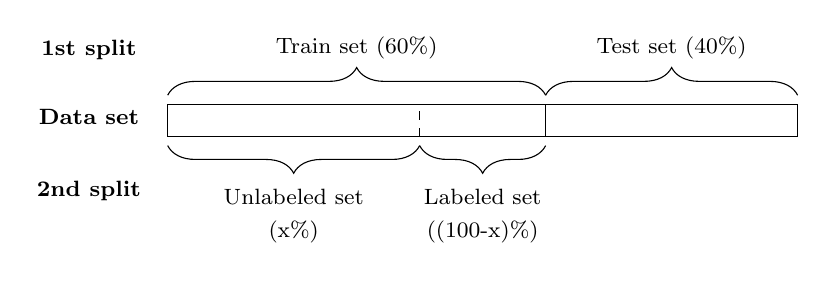
\begin{tikzpicture}[scale=0.8]
		\draw (0,0) rectangle (10,.5) node[midway]{};
		\draw (6,0) -- (6,.5);
		\draw[dashed] (4,0) -- (4,.5);
		
		\draw node[draw=none, xshift=-1cm, yshift=1.1cm] {\footnotesize \textbf{1st split}};
		\draw node[draw=none, xshift=-1cm, yshift=-.7cm] {\footnotesize \textbf{2nd split}};
		\draw node[draw=none, xshift=-1cm, yshift=.25cm] {\textbf{\footnotesize Data set}};
		
		\draw [decorate,decoration={brace,amplitude=10pt}, yshift=0.15cm]
		(0,.5) -- (6,.5) node [black,midway,yshift=0.6cm] {\footnotesize Train set (60\%)};
		\draw [decorate,decoration={brace,amplitude=10pt}, yshift=0.15cm]
		(6,.5) -- (10,.5) node [black,midway,yshift=0.6cm] {\footnotesize Test set (40\%)};
		
		\draw [decorate,decoration={brace,amplitude=10pt, mirror}, , yshift=-0.15cm]
		(0,0) -- (4,0) node [black,midway,yshift=-0.9cm, align=center] {\footnotesize Unlabeled set \\\footnotesize (x\%)};
		\draw [decorate,decoration={brace,amplitude=10pt, mirror}, yshift=-0.15cm]
		(4,0) -- (6,0) node [black,midway,yshift=-0.9cm, align=center] {\footnotesize Labeled set \\\footnotesize ((100-x)\%)};
	\end{tikzpicture}
	\caption{The split-x process in a specific data case for multinomial models.}
	\label{fig2: data preparing process}
\end{figure}

The experiments were examined with supervised multinomial Naive Bayes (NB) and the corresponding semi-supervised model with three different initialization methods. They are the conventional randomized (EM-random), hierarchical tree (EM-tree) and k-means clustering (EM-kmeans) assignments. The search component numbers are in $[1, 15]$. Ultimately, we have 3 data cases with 4 inference models -- $(3 \times 4) = 12$ classifiers. Since the results are mostly balanced between precision and recall criteria, we only show the measurement of f1-score here. Accordingly, table \ref{table2: exp news 1}, \ref{table2: exp news 2} and \ref{table2: exp news 3} present the results on comp versus rec, comp versus sci and comp versus talk respectively. The complete table of experimental results can be found in appendix \ref{appx: Experiments Resources}.

In all of the data cases and splits, we can observe that the semi-supervised models outperform the supervised NB model. We now consider only the different component initialization methods of semi-supervised classifiers. Starting with the split-70, the performance between the clustering assignments---EM-tree and EM-kmeans---and randomized assignment---EM-random---are merely the same. It is better in some cases, table \ref{table2: exp news 1}, but lower or equal in the others, and the differences are small. The same situation is also in split-90. Finally, with a narrow source of labeled data in split-97, it gives us more clarity to see the advantage of clustering assignment over the random method. Where in most of the cases, we have the better performances in EM-tree and EM-kmeans. In addition, we may notice that in all of the setup, the models show a good adaption with the changes of unlabeled data. In different scales, the classifiers still keep it performance with a small variances.

\pagebreak

\begin{table}[t!]
	\centering
	\captionsetup{justification=centering}
	\caption{Multinomial model evaluation, 20Newsgroups data, \\f1-score measurement, comp versus rec.}
	\makebox[\textwidth][c]{
		\begin{tabular}{ c|cccc }
			Label & \textbf{NB} & \textbf{EM-random} & \textbf{EM-tree} & \textbf{EM-kmeans} \\
			\hline
			
			\multicolumn{1}{c}{} & \multicolumn{4}{c}{Split-70, labeled:unlabeled = 1064:2484} \\
			\hline
			$- 1$ & 0.83 & 0.86 & 0.87 & 0.87 \\
			$+ 1$ & 0.77 & 0.79 & 0.82 & 0.81 \\
			\cline{1-5}
			avg.  & 0.80 & 0.82 & 0.85 & 0.84 \\
			\hline
			
			\multicolumn{1}{c}{} & \multicolumn{4}{c}{Split-90, labeled:unlabeled = 354:3194} \\
			\hline
			$- 1$ & 0.78 & 0.86 & 0.86 & 0.86 \\
			$+ 1$& 0.77 & 0.80 & 0.80 & 0.80 \\
			\cline{1-5}
			avg.  & 0.78 & 0.83 & 0.83 & 0.83 \\
			\hline
			
			\multicolumn{1}{c}{} & \multicolumn{4}{c}{Split-97, labeled:unlabeled = 106:3442} \\
			\hline
			$- 1$ & 0.67 & 0.77 & 0.83 & 0.78 \\
			$+ 1$ & 0.66 & 0.70 & 0.72 & 0.76 \\
			\cline{1-5}
			avg.  & 0.66 & 0.74 & 0.77 & 0.77 \\
			\hline
	\end{tabular}}
	\label{table2: exp news 1}
\end{table}

\begin{table}[t!]
	\centering
	\captionsetup{justification=centering}
	\caption{Multinomial model evaluation, 20Newsgroups data, \\f1-score measurement, comp versus sci.}
	\makebox[\textwidth][c]{
		\begin{tabular}{ c|cccc }
			Label & \textbf{NB} & \textbf{EM-random} & \textbf{EM-tree} & \textbf{EM-kmeans} \\
			\hline
			
			\multicolumn{1}{c}{} & \multicolumn{4}{c}{Split-70, labeled:unlabeled = 1061:2476} \\
			\hline
			$- 1$ & 0.90 & 0.92 & 0.92 & 0.92 \\
			$+ 1$ & 0.85 & 0.89 & 0.89 & 0.89 \\
			\cline{1-5}
			avg. & 0.88 & 0.91 & 0.91 & 0.90 \\
			\hline
			
			\multicolumn{1}{c}{} & \multicolumn{4}{c}{Split-90, labeled:unlabeled = 353:3184} \\
			\hline
			$- 1$ & 0.91 & 0.92 & 0.91 & 0.91 \\
			$+ 1$ & 0.88 & 0.89 & 0.89 & 0.89 \\
			\cline{1-5}
			avg. & 0.89 & 0.90 & 0.90 & 0.90 \\
			\hline
			
			\multicolumn{1}{c}{} & \multicolumn{4}{c}{Split-97, labeled:unlabeled = 106:3431} \\
			\hline
			$- 1$ & 0.88 & 0.89 & 0.91 & 0.91 \\
			$+ 1$ & 0.83 & 0.82 & 0.88 & 0.88 \\
			\cline{1-5}
			avg. & 0.86 & 0.86 & 0.89 & 0.89 \\
			\hline
	\end{tabular}}
	\label{table2: exp news 2}
\end{table}

\begin{table}[t!]
	\centering
	\captionsetup{justification=centering}
	\caption{Multinomial model evaluation, 20Newsgroups data, \\f1-score measurement, comp versus talk.}
	\makebox[\textwidth][c]{
		\begin{tabular}{ c|cccc }
			Label & \textbf{NB} & \textbf{EM-random} & \textbf{EM-tree} & \textbf{EM-kmeans} \\
			\hline
			
			\multicolumn{1}{c}{} & \multicolumn{4}{c}{Split-70, labeled:unlabeled = 977:2280} \\
			\hline
			$- 1$ & 0.94 & 0.95 & 0.94 & 0.95 \\
			$+ 1$ & 0.91 & 0.91 & 0.91 & 0.91 \\
			\cline{1-5}
			avg. & 0.93 & 0.93 & 0.93 & 0.93 \\
			\hline
			
			\multicolumn{1}{c}{} & \multicolumn{4}{c}{Split-90, labeled:unlabeled = 325:2932} \\
			\hline
			$- 1$ & 0.94 & 0.94 & 0.94 & 0.94 \\
			$+ 1$ & 0.89 & 0.91 & 0.90 & 0.91 \\
			\cline{1-5}
			avg. & 0.91 & 0.93 & 0.92 & 0.93 \\
			\hline
			
			\multicolumn{1}{c}{} & \multicolumn{4}{c}{Split-97, labeled:unlabeled = 97:3160} \\
			\hline
			$- 1$ & 0.91 & 0.93 & 0.94 & 0.94 \\
			$+ 1$ & 0.84 & 0.87 & 0.91 & 0.91 \\
			\cline{1-5}
			avg. & 0.88 & 0.90 & 0.92 & 0.92 \\
			\hline
	\end{tabular}}
	\label{table2: exp news 3}
\end{table}